\documentclass[a4paper,twoside]{article}
\usepackage[T1]{fontenc}
\usepackage[bahasa]{babel}
\usepackage{graphicx}
\usepackage{graphics}
\usepackage{float}
\usepackage[cm]{fullpage}
\pagestyle{myheadings}
\usepackage{etoolbox}
\usepackage{setspace} 
\usepackage{lipsum} 
\setlength{\headsep}{30pt}
\usepackage[inner=2cm,outer=2.5cm,top=2.5cm,bottom=2cm]{geometry} %margin
% \pagestyle{empty}

\makeatletter
\renewcommand{\@maketitle} {\begin{center} {\LARGE \textbf{ \textsc{\@title}} \par} \bigskip {\large \textbf{\textsc{\@author}} }\end{center} }
\renewcommand{\thispagestyle}[1]{}
\markright{\textbf{\textsc{Laporan Perkembangan Pengerjaan Skripsi\textemdash Sem. Genap 2017/2018}}}

\onehalfspacing
 
\begin{document}

\title{\@judultopik}
\author{\nama \textendash \@npm} 

%ISILAH DATA BERIKUT INI:
\newcommand{\nama}{Vanessa Sukamto}
\newcommand{\@npm}{2014730010}
\newcommand{\tanggal}{25/04/2018} %Tanggal pembuatan dokumen
\newcommand{\@judultopik}{Simulator Pertumbuhan Wirausaha Berbasis Cellular Automata} % Judul/topik anda
\newcommand{\kodetopik}{CEN4402}
\newcommand{\jumpemb}{1} % Jumlah pembimbing, 1 atau 2
\newcommand{\pembA}{Cecilia Esti Nugraheni}
\newcommand{\pembB}{-}
\newcommand{\semesterPertama}{8 - Genap 17/18} % semester pertama kali topik diambil, angka 1 dimulai dari sem Ganjil 96/97
\newcommand{\lamaSkripsi}{1} % Jumlah semester untuk mengerjakan skripsi s.d. dokumen ini dibuat
\newcommand{\kulPertama}{Skripsi 1} % Kuliah dimana topik ini diambil pertama kali
\newcommand{\tipePR}{B} % tipe progress report :
% A : dokumen pendukung untuk pengambilan ke-2 di Skripsi 1
% B : dokumen untuk reviewer pada presentasi dan review Skripsi 1
% C : dokumen pendukung untuk pengambilan ke-2 di Skripsi 2

% Dokumen hasil template ini harus dicetak bolak-balik !!!!

\maketitle

\pagenumbering{arabic}

\section{Data Skripsi} %TIDAK PERLU MENGUBAH BAGIAN INI !!!
Pembimbing utama/tunggal: {\bf \pembA}\\
Pembimbing pendamping: {\bf \pembB}\\
Kode Topik : {\bf \kodetopik}\\
Topik ini sudah dikerjakan selama : {\bf \lamaSkripsi} semester\\
Pengambilan pertama kali topik ini pada : Semester {\bf \semesterPertama} \\
Pengambilan pertama kali topik ini di kuliah : {\bf \kulPertama} \\
Tipe Laporan : {\bf \tipePR} -
\ifdefstring{\tipePR}{A}{
			Dokumen pendukung untuk {\BF pengambilan ke-2 di Skripsi 1} }
		{
		\ifdefstring{\tipePR}{B} {
				Dokumen untuk reviewer pada presentasi dan {\bf review Skripsi 1}}
			{	Dokumen pendukung untuk {\bf pengambilan ke-2 di Skripsi 2}}
		}
		
\section{Latar Belakang}

Pada saat ini, lapangan kerja pada suatu negara tidak bisa kita prediksi, tetapi kenyataan yang kita ketahui adalah lapangan kerja dari tahun ke tahun semakin terbatas. Dengan melihat situasi tersebut maka bisa dipastikan tingkat pengangguran di suatu negara akan semakin tinggi. Solusi terbaik untuk mengurangi permasalahan tersebut adalah dengan berwirausaha. Kewirausahaan adalah kemampuan seseorang untuk membuat suatu usaha yang dimulai dari 0 atau dimulai dari bawah yang dirintis hingga usaha tersebut benar-benar sukses. Tentu saja hal ini memberikan pengaruh positif terhadap pertumbuhan ekonomi suatu negara, karena kewirausahaan juga sekaligus membuka lapangan kerja bagi masyarakat. Jika usaha yang dirintis semakin besar, otomatis perusahaan tersebut akan merekrut tenaga kerja yang semakin banyak lagi. 

 
Pada jaman sekarang, sudah banyak sekali orang yang lebih memilih untuk berwirausaha daripada bekerja di kantor atau di sebuah perusahaan. Alasan mengapa banyak orang lebih memilih berwirausaha pun bervariasi contohnya orang tersebut tidak terlalu menyukai waktu kerjanya diatur oleh orang lain melainkan ia lebih menyukai waktu kerjanya diatur oleh dirinya sendiri. Tidak hanya pada jaman sekarang, dari jaman dahulu juga sudah ada wirausaha yang namanya tidak asing lagi didengar oleh telinga kita salah satunya yaitu Bob Sadino. Untuk menjadi wirausaha yang sukses seperti Bob Sadino tidaklah mudah, pasti ada beberapa faktor dari luar maupun dalam yang mempengaruhi keberlangsungan wirausaha. Dalam berwirausaha dibutuhkan usaha yang besar untuk menjadi sukses, usaha tersebut juga harus dijaga kekonsistenannya agar tidak mengalami kebangkrutan.


Kewirausahaan sangat diperlukan guna mendorong perekonomian suatu negara karena dapat mengurangi tingkat pengangguran di Indonesia. Secara ekonomis, kewirausahaan akan membantu meningkatkan pendapatan masyarakat atau meningkatkan kesejahteraan melalui penciptaan produk baru, serta mengurangi kemiskinan.  Ideal besarnya populasi wirausaha dalam suatu negara adalah 2\% dari total penduduk suatu negara. Saat ini Indonesia baru mencapai pengusaha dari total penduduk. Maka dari itu, kondisi wirausaha ini perlu dipantau terus-menerus perkembangannya agar dapat memajukan perekonomian di Indonesia. Pemantauan ini dilakukan oleh pemerintah dan lembaga-lembaga swasta yang berkepentingan. Salah satu lembaga yang memantau adalah GEM (Global Entrepreneurship Monitor). GEM merupakan konsorsium yang bertujuan untuk mengukur dan memantau kegiatan kewirausahaan. 


GEM mengilustrasikan kewirausahaan menjadi 3 fase, fase pertama yaitu wirausaha \textit{nascent}, yaitu mereka yang baru memulai suatu usaha (<3 bulan). Fase kedua yaitu pemilik usaha baru (\textit{new business owners}), yaitu wirausaha \textit{nascent} yang sudah menjalani usaha lebih dari tiga bulan tetapi tidak lebih dari tiga setengah tahun. Fase ketiga yaitu wirausaha mapan (\textit{established entrepreneurs}), yaitu wirausaha yang sudah menjalankan sebuah usaha lebih dari tiga setengah tahun.


Selain pemantauan terhadap kondisi riil, salah satu kegiatan yang mendukung pemantauan adalah pengamatan secara tidak langsung. Salah satu pengamatan tidak langsung adalah dengan membuat model matematika dari pertumbuhan wirausaha dan kemudian melakukan simulasi terhadap model tersebut. Salah satu model matematika yang dapat digunakan untuk memodelkan pertumbuhan wirausaha adalah Entrepreneurial Cellular Automata (ECA) yang diusulkan oleh Nugraheni dan Natali. ECA adalah pengembangan dari Cellular Automata standar dari Ulam dan New Neuman. Cellular Automata (CA) sendiri merupakan suatu model matematika yang digunakan untuk memodelkan suatu sistem dinamis. Pada ECA dijelaskan bagaimana struktur dari ECA dan diberikan illustrasi bagaimana menggunakan ECA untuk memprediksi pertumbuhan wirausaha berdasarkan parameter wirausaha dari GEM. 


Dalam hasil penelitian ECA setiap wirausahawan mempunyai beberapa atribut yang bersifat statis maupun dinamis. Contoh atribut yang bersifat statis yaitu bidang usaha, kategori usaha, lokasi geografis dan jenis kelamin. Sementara contoh untuk atribut dinamis adalah usia, level wirausaha dan usia usaha. Diantara atribut dinamis, level wirausaha menjadi atribut penting karena atribut ini yang akan menjadi acuan untuk menentukan perkembangan dari kewirausahaan. \textit{Continuity Index} digunakan untuk menentukan apakah seorang wirausahawan pada suatu saat tertentu akan meneruskan usahanya pada waktu selanjutnya.


Skripsi ini bertujuan untuk mengembangkan ECA dengan memperhitungkan beberapa parameter yang belum diperhatikan pada ECA dan mengembangkan perangkat lunak simulator yang dapat menampilkan visualisasi dari simulasi. Selain menambahkan parameter yang berhubungan dengan pertumbuhan wirausaha, pengembangan ini juga akan memperhatikan pertumbuhan penduduk. Di samping itu, simulasi pada data nyata juga perlu dilakukan untuk membuktikan kebenaran dari model yang dibuat.


\section{Tujuan}

Berdasarkan rumusan masalah yang telah dibuat, maka tujuan penelitian ini dijelaskan ke dalam poin-poin sebagai berikut :


\begin{enumerate}
	\item Mempelajari faktor yang berpengaruh pada keberlangsungan wirausaha.
	\item Memodelkan pertumbuhan wirausaha dengan \textit{cellular automata}.
	\item Mengembangkan model keberlangsungan wirausaha dengan \textit{cellular automata}.
\end{enumerate}

\section{Rumusan Masalah}

Berikut adalah susunan permasalahan yang akan dibahas pada penelitian ini:


\begin{enumerate}
	\item Faktor apa saja yang mempengaruhi keberlangsungan wirausaha?
	\item Bagaimana memodelkan pertumbuhan wirausaha dengan \textit{cellular automata} ?
	\item Bagaimana mengembangkan model keberlangsungan wirausaha dengan \textit{cellular automata}?
\end{enumerate}

\section{Detail Perkembangan Pengerjaan Skripsi}
Detail bagian pekerjaan skripsi sesuai dengan rencana kerja/laporan perkembangan terakhir :
	\begin{enumerate}
		\item Mempelajari kewirausahaan secara umum khususnya GEM.
		
		
		{\bf Status :} Ada sejak rencana kerja skripsi.\\
		{\bf Hasil :} 
		Menurut penelitian GEM, kewirausahaan dibagi menjadi beberapa tahapan. Pertama, individu yang mulai terlibat dalam dunia kewirausahaan yang memiliki kemampuan untuk membuka usaha, mampu melihat peluang dan tidak takut akan kegagalan dalam membuka suatu usaha (\textit{Potential Entrepreneur}). Kedua, individu yang sudah menjalankan usahanya dalam waktu kurang dari tiga bulan (\textit{Nascent Entrepreneur}). Ketiga, individu yang sudah menjalankan usahanya lebih dari tiga bulan tetapi kurang dari tiga setengah tahun (\textit{New Business Owners}). Wirausaha \textit{nascent} dan \textit{New Business Owners} ini masuk dalam TEA (Totally Early-Stage Entrepreneurial Activity) dalam sebuah ekonomi. Tahapan terakhir yaitu individu yang sudah menjalankan usahanya lebih dari tiga setengah tahun (\textit{Established Entrepreneurs}).
		
\begin{figure} [H]
	\centering  
	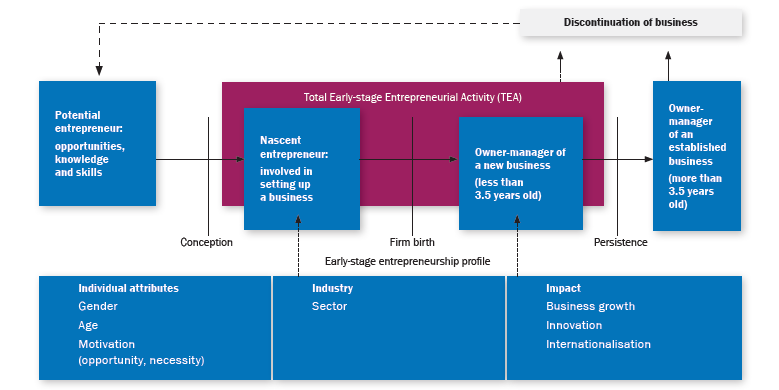
\includegraphics[width=16cm, height=8cm]{GEM2016-wirausaha}  
	\caption[Fase Wirausaha]{Fase Wirausaha} 
	\label{fig:fasewirausaha} 
\end{figure}
		

Tahapan dari wirausaha juga dipengaruhi oleh atribut internal dari wirausahawan itu sendiri dalam menjalankan usahanya. Atribut-atribut ini dibedakan menjadi atribut statis (nilainya tidak berubah) dan atribut dinamis (nilainya dapat berubah). Berikut merupakan atribut-atribut yang mempengaruhi berlangsungnya kegiatan kewirausahaan:
			\begin{enumerate}
				\item Atribut Dinamis
					\begin{itemize}
						\item Umur : usia dari wirausaha itu sendiri.
						\item Level Wirausaha : tingkat wirausaha dilihat dari berapa lama usaha itu dilakukan.
						\item Usia usaha : usia dari usaha yang dilakukan wirausahawan.
					\end{itemize}
				\item Atribut Statis
					\begin{itemize}
						\item Bidang usaha : bidang usaha yang ditekuni oleh wirausahawan.
						\item Kategori usaha : kategori usaha yang dipilih oleh wirausahawan (kecil,menengah dan besar).
						\item Jenis kelamin : jenis kelamin wirausahawan tersebut.
						\item Lokasi geografis : lokasi berdirinya usaha tersebut.
					\end{itemize}
			\end{enumerate}


Terdapat juga indikator-indikator berdasarkan faktor psikologi individu yang menjalankan usaha. Untuk lebih jelasnya dapat dilihat pada tabel \ref{tabelindikator} :

\begin{table}[H]
\centering
\caption{Tabel Indikator GEM}
\begin{tabular}{|p{4cm}|p{12cm}|}
\hline
Indikator & Deskripsi\\
\hline
Perceived Opportunities & Persentase penduduk antara usia 18-64 tahun yang melihat peluang baik untuk memulai usaha. \\
\hline
Perceived Capabilities & Persentase penduduk antara usia 18-64 tahun yang percaya bahwa mereka mempunyai kemampuan untuk memulai suatu usaha. \\
\hline
Entreprenurial Intention & Persentase penduduk antara usia 18-64 tahun (selain orang yang berwirausaha) yang bertekad untuk mendirikan usaha dalam waktu tiga tahun kedepan.\\
\hline
Fear of Failure Rate & Persentase penduduk antara usia 18-64 tahun dapat melihat peluang baik yang mengindikasikan bahwa takut akan gagal akan menjauhkan mereka dari mendirikan usaha. \\
\hline
Role Model & Persentase penduduk antara usia 18-64 tahun yang memulai bisnis pada dua tahun terakhir.\\
\hline
New Product Early-Stage Entrepreneurial (TEA) Activity & Persentase dari TEA yang mengindikasikan bahwa produk atau jasa mereka masih baru (untuk beberapa konsumen).\\
\hline
Growth Expectation Early-stage Entrepreneurial Activity : Relative Prevalence & Persentase dari TEA yang berharap untuk mempekerjakan paling sedikit lima karyawan dalam waktu lima tahun kedepan\\
\hline
Informal Investors Rate & Persentase dari populasi berusia 18-64 yang telah menyediakan dana untuk sebuah usaha baru, didirikan oleh orang lain dalam waktu tiga tahun terakhir.\\
\hline
Totaly Early-stage Entrepreneurial Activity for Female Working Age Population & Persentase dari populasi wanita berusia 18-64 yang merupakan seorang wirausaha nascent (pemilik usaha baru).\\
\hline
Totaly Early-stage Entrepreneurial Activity for Male Working Age Population & Persentase dari populasi pria berusia 18-64 yang merupakan seorang wirausaha nascent (pemilik usaha baru).\\
\hline
Improvement-Driven Opportunity Entrepreneurial Activity : Relative Prevalence & persentase orang yang terlibat dalam TEA yang mengklaim bahwa mereka didorong oleh kesempatan bukan karena kurangnya pilihan pekerjaan\\
\hline
Necessity-Driven Entrepreneurial Activity : Relative Prevalence & persentase orang yang terlibat dalam TEA yang berwirausaha karena mereka tidak punya pilihan pekerjaan lain.\\
\hline
Established Business Ownership Rate & Persentase dari populasi berusia 18-64 yang merupakan pemilik manager dari sebuah usaha mapan dan sudah menghasilkan gaji atau untung apapun ke pemiliknya selama lebih dari 42 bulan.\\
\hline
Total Early-stage Entrepreneurial Activity & persentase dari populasi berusia 18-64 yang merupakan wirausaha nascent.\\
\hline
New Business Ownership Rate & Persentase dari populasi 18-64 yang merupakan pemilik manager dari sebuah usaha mapan yang sudah menghasilkan gaji atau untung selama lebih dari 3 bulan tetapi tidak lebih dari 42 bulan.\\
\hline
Nascent Entrepreneurship Rate & Persentase dari populasi 18-64 yang merupakan wirausaha nascent terlibat secara aktif memulai suatu usaha yang mereka miliki sendiri/bersama.\\
\hline
Media Attention for Entrepreneurship & persentase dari populasi berusia 18-64 yang setuju dengan pernyataan bahwa di negara mereka, mereka sering melihat atau mendengar di media tentang usaha baru yang sukses.\\
\hline
High status successful Entrepreneur & persentase dari populasi berusia 18-64 yang setuju dengan pernyataan bahwa di negara mereka, wirausaha yang sukses dihormati dan bercitra tinggi.\\
\hline
Entrepreneurship as Desirable Care & persentase dari populasi berusia 18-64 yang setuju dengan pernyataan bahwa di negara mereka, kebanyakan orang mempertimbangkan untuk memulai usaha baru sebagai karir yang diinginkan.\\
\hline
Know Startup Entrepreneur Rate & persentase dari populasi berusia 18-64 yang kenal seseorang yang mendirikan suatu usaha dalam waktu 2 tahun terakhir secara pribadi.\\
\hline
\end{tabular}
\label{tabelindikator}
\end{table}


Setelah mempelajari tentang atribut dan indikator-indikator dalam berwirausaha, berikut merupakan data nyata dari GEM berdasarkan beberapa indikator. Pertama, data pendidikan di Indonesia dari GEM tentang Perceived Capabilities yang diambil pada tahun 2015.

\begin{figure} [H]
	\centering  
	\includegraphics[width=14cm, height=7cm]{PCPendidikan} 
	\caption[Komposisi perceived capabilities untuk tingkat pendidikan yang berbeda]{Komposisi perceived capabilities untuk tingkat pendidikan yang berbeda} 
	\label{fig:PCPendidikan} 
\end{figure}

Dapat dilihat pada gambar \ref{fig:PCPendidikan} dijelaskan bahwa individu yang memiliki kemampuan berwirausaha tertinggi yaitu pada individu yang berpendidikan sekolah menengah ke atas (SMA). Pria mempunyai peluang yang lebih unggul (58.5\%) daripada wanita (55.4\%). Peluang yang paling rendah untuk menjadi wirausaha yaitu pada individu yang berpendidikan sampai S-3 yaitu 0.0\% untuk wanita dan 0.1\% untuk pria. 

\begin{figure} [H]
	\centering  
	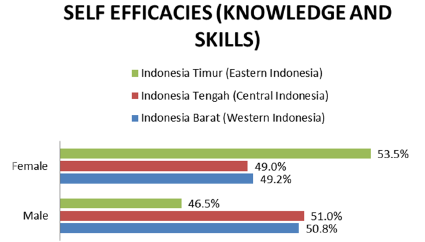
\includegraphics[width=11cm, height=6cm]{PCRegion} 
	\caption[Komposisi perceived capabilities untuk wilayah Indonesia]{Komposisi perceived capabilities untuk wilayah Indonesia} 
	\label{fig:PCRegion} 
\end{figure}

Dapat dilihat pada gambar \ref{fig:PCRegion} dijelaskan bahwa individu yang memiliki kemampuan berwirausaha tertinggi yaitu pada wanita yang berada pada wilayah Indonesia Timur sebesar 53.5\% sedangkan pria yang berpeluang tinggi untuk menjadi wirausaha berada pada wilayah Indonesia Tengah sebesar 51.0\%. Individu yang memiliki kemampuan berwirausaha terendah yaitu untuk wanita berada pada wilayah Indonesia Tengah sebesar 49.0\% dan untuk pria berada pada wilayah Indonesia Timur sebesar 46.5\%. Data kedua yaitu data Role Model tentang perbedaan tingkat wirausaha antara perempuan dan laki-laki serta yang kedua adalah data pendidikan.

\begin{figure} [H]
	\centering  
	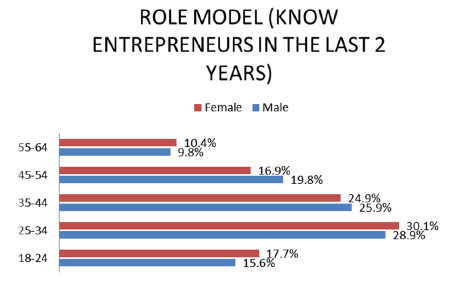
\includegraphics[width=12cm, height=7cm]{RMfemalemale} 
	\caption[Komposisi role model untuk wanita dan pria]{Komposisi role model untuk wanita dan pria} 
	\label{fig:RMfemalemale} 
\end{figure}


Pada gambar \ref{fig:RMfemalemale} dijelaskan individu yang memulai bisnis dalam 2 tahun terakhir. Peluang individu yang memulai bisnis dalam 2 tahun terakhir tertinggi yaitu pada wanita usia 25 sampai 34 tahun sebesar 30.1\% sedangkan pria sebesar 28.9\%. Peluang terendah yaitu pada wanita usia 55 sampai 64 tahun sebesar 10.4\% sedangkan pria sebesar 9.8\%.


\begin{figure} [H]
	\centering  
	\includegraphics[width=13cm, height=7cm]{RMpendidikan} 
	\caption[Komposisi role model untuk tingkat pendidikan yang berbeda]{Komposisi role model untuk tingkat pendidikan yang berbeda} 
	\label{fig:RMpendidikan} 
\end{figure}  


Pada gambar \ref{fig:RMpendidikan} dijelaskan individu yang memulai bisnis dalam 2 tahun terakhir. Peluang individu yang memulai bisnis dalam 2 tahun terakhir tertinggi pada individu yang mempunyai tingkat pendidikan sekolah menengah ke atas (SMA). Pria memperoleh persentase sebesar 58.3\% dan wanita sebesar 54.4\%. Individu yang mempunyai peluang terendah yaitu individu yang berpendidikan S-3. Pria memperoleh persentase sebesar 0.1\% dan wanita memperoleh persentase sebesar 0.0\%. Data ketiga yaitu data Perceived Opportunities tentang perbedaan tingkat wirausaha antara perempuan dan laki-laki serta yang kedua adalah data pendidikan.

\begin{figure} [H]
	\centering  
	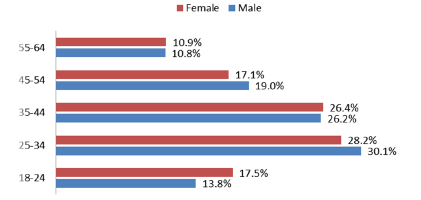
\includegraphics[width=12cm, height=6cm]{POfemalemale} 
	\caption[Komposisi role model untuk wanita dan pria]{Komposisi role model untuk wanita dan pria} 
	\label{fig:POfemalemale} 
\end{figure} 

Pada gambar \ref{fig:POfemalemale} dijelaskan kemampuan individu antara pria dan wanita dalam melihat peluang berwirausaha. Peluang tertinggi yaitu pada pria berusia 25 sampai 34 tahun yang memiliki persentase sebesar 30.1\% dan wanita sebesar 28.2\%. Peluang terendah yaitu pada pria berusia 55 sampai 64 tahun sebesar 10.8\% dan wanita sebesar 10.9\%. 

\begin{figure} [H]
	\centering  
	\includegraphics[width=14cm, height=6cm]{POpendidikan} 
	\caption[Komposisi perceived opportunities untuk tingkat pendidikan yang berbeda]{Komposisi perceived opportunities untuk tingkat pendidikan yang berbeda} 
	\label{fig:POpendidikan} 
\end{figure}  

Gambar \ref{fig:POpendidikan} menjelaskan kemampuan individu dalam melihat peluang. Kemampuan melihat peluang berwirausaha tertinggi yaitu pada individu yang berpendidikan sekolah menengah ke atas (SMA). Persentase pria sebesar 59.3\% dan wanita sebesar 56.7\%. Kemampuan melihat peluang berwirausaha terendah yaitu pada individu yang berpendidikan S-3. Persentase pria sebesar 0.2\% dan wanita sebesar 0.0\%. Data keempat yaitu data Fear of Failure tentang perbedaan tingkat wirausaha antara perempuan dan laki-laki.

\begin{figure} [H]
	\centering  
	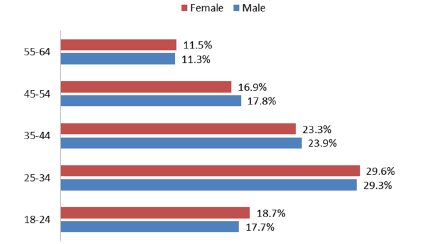
\includegraphics[width=13cm, height=6cm]{FOFfemalemale} 
	\caption[Komposisi fear of failure untuk wanita dan pria]{Komposisi fear of failure untuk wanita dan pria} 
	\label{fig:FOF} 
\end{figure}  

Gambar \ref{fig:FOF} menjelaskan perbedaan Fear of Failure antara pria dan wanita. Persentase Fear of Failure yang tertinggi yaitu pada wanita berusia 25 sampai 34 tahun sebesar 29.6\% dan pria sebesar 29.3\%. Persentase Fear of Failure terendah yaitu pada wanita usia 55 sampai 64 tahun sebesar 11.5\% dan pria sebesar 11.3\%. 

	\item Mempelajari teori tentang \textit{Cellular Automata} yang khususnya \textit{Entrepreneur Cellular Automata} (ECA).
	
	
	  {\bf Status :} Ada sejak rencana kerja skripsi.\\
		{\bf Hasil :}
		
		Cellular automata (CA) adalah model matematis untuk sistem dimana banyak komponen sederhana yang bertindak secara bersamaan untuk menghasilkan pola perilaku yang rumit. Sebuah CA terdiri atas sekumpulan sel yang tersusun dalam larik-larik (\textit{grid}). Setiap sel mempunyai kondisi (\textit{state}) tertentu dan dapat berubah sesuai dengan aturan tertentu. Perubahan \textit{state} dari sebuah sel dipengaruhi oleh sel disekitarnya atau disebut dengan sel tetangga.
		\begin{enumerate}
			\item Dimensi pada CA
			 \begin{itemize}
			  \item CA Satu Dimensi
			
				\begin{figure} [H]
					\centering  
					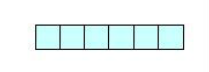
\includegraphics[width=4cm, height=2cm]{CA1D} 
					\caption[CA 1 Dimensi]{CA 1 Dimensi} 
					\label{fig:CA1D} 
				\end{figure}
			
			Cellular Automata satu dimensi adalah cellular automata yang ruang selnya berupa array satu dimensi, sehingga masing-masing sel hanya memiliki dua tetangga yang tepat bersebelahan, kecuali sel paling pinggir yang hanya mempunyai satu tetangga. CA satu dimensi biasanya memakai aturan yang diusulkan oleh Wolfram. Sebagai contoh berikut aturan no. 30 diberikan pada gambar \ref{fig:wolfram}
			
			
			\begin{figure} [H]
					\centering  
					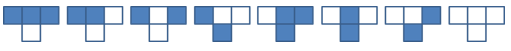
\includegraphics[width=10cm, height=2cm]{wolfram} 
					\caption[Aturan 30 dari Wolfram]{Aturan 30 dari Wolfram} 
					\label{fig:wolfram} 
				\end{figure}
				
				Cara membaca aturan tersebut adalah pada baris pertama terdapat 3 sel pada suatu saat (iterasi) tertentu, sel yang ditinjau adalah sel yang berada di tengah. Tetangga dari sel tersebut yaitu tetangga kiri dan kanan. Baris kedua menunjukkan keadaan sel pada \textit{state} berikutnya. Sebagai contoh pada gambar paling kiri, sel pada bagian tengah (gelap) mempunyai tetangga kiri gelap dan tetangga kanan gelap maka iterasi berikutnya \textit{state} sel tersebut berubah menjadi putih.
				
				Sebagai ilustrasi, pada gambar \ref{fig:penerapanwolfram} diberikan contoh penerapan aturan 30 dari Wolfram yang dimulai dari kondisi awal (t=0) dengan sel gelap yang berada di tengah hingga t=9. \cite{ECA}
				
				\begin{figure} [H]
					\centering  
					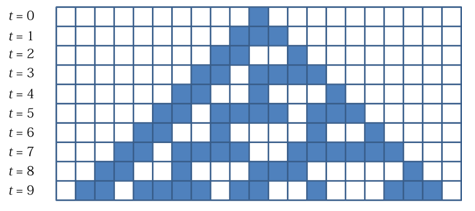
\includegraphics[width=10cm, height=6cm]{penerapanwolfram} 
					\caption[Ilustrasi penerapan aturan 30 dari Wolfram]{Ilustrasi penerapan aturan 30 dari Wolfram} 
					\label{fig:penerapanwolfram} 
				\end{figure}
				
			  \item CA Dua Dimensi
			
			\begin{figure} [H]
					\centering  
					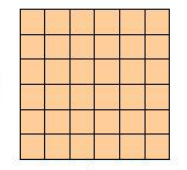
\includegraphics[width=4cm, height=2cm]{CA2D} 
					\caption[CA 2 Dimensi]{CA 2 Dimensi} 
					\label{fig:CA2D} 
				\end{figure}
			
			Cellular Automata dua dimensi adalah cellular automata yang ruang selnya biasanya berupa matriks, sehingga masing-masing sel memiliki lebih dari dua tetangga. CA dua dimensi yang sangat terkenal adalah Conway's \textit{Game of Life}. Setiap sel pada CA menggambarkan suatu individu yang dapat berada pada \textit{state} hidup atau mati. Sel hidup dapat berubah menjadi mati dan sel mati dapat berubah menjadi sel hidup. Aturan dasar Conway's diberikan pada gambar \ref{fig:conway}
			
			
			\begin{figure} [H]
					\centering  
					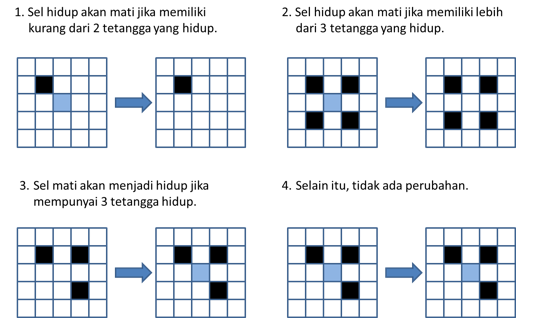
\includegraphics[width=12cm, height=8cm]{conway} 
					\caption[Aturan Dasar Conway's Game of Life]{Aturan Dasar Conway's Game of Life} 
					\label{fig:conway} 
				\end{figure}
			
			Berikut ilustrasi Conway yang menggambarkan perubahan yang terjadi pada sekumpulan sel mulai dari kondisi awal (t=0) sampai dengan kondisi akhir (t=3) yang dilakukan secara iteratif. Banyaknya sel hidup pada kondisi awal berkurang sedikit demi sedikit sampai pada kondisi akhir tidak ada lagi sel hidup. \cite{ECA}
			
			
			\begin{figure} [H]
					\centering  
					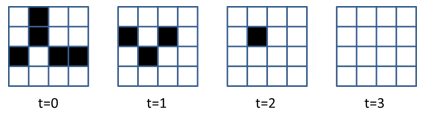
\includegraphics[width=10cm, height=3cm]{contohconway} 
					\caption[Ilustrasi Conway's Game of Life]{Ilustrasi Conway's Game of Life} 
					\label{fig:contohconway} 
				\end{figure}
				%\end{enumerate}
			\end{itemize}
			\item Aplikasi CA
			
			
			CA juga banyak digunakan untuk membantu kehidupan sehari-hari. Seperti misalnya penerapan CA pada bidang transportasi, yaitu pengaturan lampu lalu lintas. Model dalam penelitian ini menggunakan CA satu dimensi. Penerapan CA lainnya yaitu pada bidang kesehatan, yaitu simulasi infeksi virus influenza A. Pada penelitian ini digunakan CA dua dimensi.
			
			
		Setelah membahas tentang CA, berikut penjelasan tentang Entrepreneurial Cellular Automata (ECA). ECA adalah pengembangan model dari Cellular Automata yang digunakan untuk mensimulasikan pertumbuhan kewirausahaan di Indonesia. Dalam kasus ECA ini sel akan merepresentasikan wirausahawan dan ketetanggaannya akan merepresentasikan hubungan antar wirausahawan. Setiap wirausahawan mempunyai atribut statis dan dinamis (seperti yang sudah dijelaskan pada GEM). Atribut penting dalam kewirausahaan ini yaitu level wirausaha karena atribut ini digunakan untuk menentukan perkembangan dari kewirausahaan. Cara menentukan seorang wirausaha akan meneruskan usahanya diketahui dari sebuah angka yang disebut \textit{Continuity Index} (\textit{CIdx}). Seorang wirausahawan akan meneruskan usahanya jika \textit{CIdx}-nya memenuhi nilai ambang tertentu.
		
		Atribut dari seorang wirausahawan dapat berubah dari waktu ke waktu, hal ini menyebabkan ketetanggaan juga dapat berubah dari waktu ke waktu. Sebagai contoh, diasumsikan terdapat wirausahawan $e1$ dan $e2$ bertetanggaan pada waktu $t$, jika $e1$ berubah keadaannya pada $t+1$ maka $e1$ dan $e2$ tidak lagi bertetanggaan pada saat $t+1$.
		
		
		Berikut definisi ECA yang berupa sebuah tupel :
		
		Diberikan \textit{p} himpunan nilai atribut: $A_{1}, ..., A_{p}$ dan sebuah indikator $Pub$ = ${p_{1}, ..., p_{m}}$, sebuah ECA $M$ adalah sebuah tupel
\begin{displaymath}
	M = (E, \alpha, N, \omega, \rho, \delta, \sigma)
\end{displaymath}
dimana :
\begin{itemize}
	\item $E = {e_{1}, ..., e_{n}}$ adalah himpunan berhingga wirausahaan,
	\item $\alpha = {\alpha_{1}, ..., \alpha_{p}}$ adalah himpunan berhingga atribut dimana setiap $\alpha_{i}$ didefinisikan sebagai $\alpha_{i} : E \rightarrow A_{i}$,
	\item $N = {N_{1}, ..., N_{k}}$ adalah himpunan berhingga ketetanggaan dimana setiap $N_{i}$ didefinisikan sebagai $N_{i}:E \times E \rightarrow \Re$,
	\item $\omega = {\omega_{1}, ..., \omega_{k}}$ adalah himpunan fungsi bobot atau nilai ketetanggaan dimana $\omega_{i} : N_{i} \rightarrow \Re$ memetakan setiap fungsi ketetanggaan ke sebuah bilangan riil,
	\item $\rho = {\rho_{1}, ..., \rho_{p}}$ adalah himpunan indikator publik dimana setiap $\rho_{i}$ didefinisikan sebagai $\rho_{i} : p_{i} \rightarrow \Re$,
	\item $\delta : \beta \rightarrow \beta$ adalah fungsi transisi state, dan
	\item $\sigma : N \rightarrow N$ adalah sebuah fungsi transformasi ketetanggaan.
\end{itemize}

Berdasarkan model kewirausahaan terdapat empat tingkatan wirausaha yaitu \textit{potential}, \textit{nascent}, \textit{new business manager} dan \textit{manager of established business}. Akan ditambahkan pula tingkatan wirausaha yang menyatakan wirausahawan di atas umur 64 tahun yaitu \textit{retired}. Pada gambar \ref{fig:tingkatwirausaha} akan ditunjukkan secara lebih lanjut, \textit{new\_bm} dan \textit{est\_bm} dinyatakan sebagai \textit{new business manager} dan \textit{manager of established business}.


	\begin{figure} [H]
		\centering  
		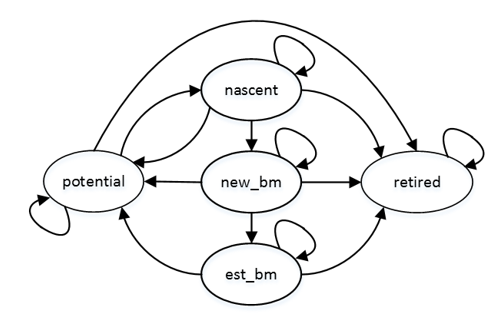
\includegraphics[width=9cm, height=5cm]{tingkatwirausaha} 
		\caption[Diagram Transisi Level Wirausaha]{Diagram Transisi Level Wirausaha} 
		\label{fig:tingkatwirausaha} 
	\end{figure}
	

Perubahan dari satu level ke level yang lain berdasarkan pada sebuah nilai yang dinamakan Continuity Index, selain usia usaha dan usia individu. Pada tabel \ref{tabelLW} akan dijelaskan mengenai transisi level dengan menggunakan lambang-lambang \textit{CIdx, bl, a ,b} dan \textit{th} untuk menyatakan \textit{Continuity Index, level} , usia individu, usia usaha dan nilai ambang. Nilai ambang ini digunakan sebagai syarat minimal yang harus dipenuhi wirausahawan untuk dapat meneruskan usahanya. Sebagai satu waktu digunakan bulan.

\begin{table}[H]
\centering
\caption{Transisi Level Wirausaha}
\begin{tabular}{|c|c|}
\hline
Waktu sekarang & Waktu berikutnya \\
\hline
\textit{bl} = potential, $ \textit{CIdx} < \textit{th}, \textit{a} < 64 \times 12$ & \textit{bl} = potential \\
\hline
\textit{bl} = potential, $\textit{CIdx} \geq \textit{th}, \textit{a} < 64 \times 12$ & \textit{bl} = nascent \\
\hline
\textit{bl} = potential, $\textit{a} \geq 64 \times 12$ & \textit{bl} = retired \\
\hline
\textit{bl} = nascent, $\textit{CIdx} < \textit{th}, \textit{a} <64 \times 12$ & \textit{bl} = potential \\
\hline
\textit{bl} = nascent, $\textit{CIdx} \geq \textit{th}, \textit{b} < 3$ & \textit{bl} = nascent \\
\hline
\textit{bl} = nascent, $\textit{a} \geq 64 \times 12$ & \textit{bl} = retired \\
\hline
\textit{bl} = new\_bm, $\textit{CIdx} < \textit{th}, \textit{a} < 64 \times 12$ & \textit{bl} = potential \\
\hline
\textit{bl} = new\_bm, $\textit{CIdx} \geq \textit{th}, \textit{b} < 42$ & \textit{bl} = potential \\
\hline
\textit{bl} = new\_bm, $\textit{a} \geq 64 \times 12$ & \textit{bl} = retired \\
\hline
\textit{bl} = est\_bm, $\textit{CIdx} < \textit{th}, \textit{a} < 64 \times 12$ & \textit{bl} = potential \\
\hline
\textit{bl} = est\_bm, $\textit{CIdx} \geq \textit{th}, \textit{a} < 64 \times 12$ & \textit{bl} = est\_bm \\
\hline
\textit{bl} = est\_bm, $\textit{a} \geq 64 \times 12$ & \textit{bl} = retired \\
\hline
\textit{bl} = retired, $\textit{a} \geq 64 \times 12$ & \textit{bl} = retired \\
\hline
\end{tabular}
\label{tabelLW}
\end{table}

Untuk memberikan gambaran bagaimana penggunaan model untuk memantau pertumbuhan wirausaha, dilakukan simulasi menggunakan data yang tidak nyata. Simulasi ini menggunakan atribut berupa umur, level wirausaha dan jenis kelamin.


%rumus CIdx
Misal $Cint_{i}(t)$ dan $Cneg_{i}(t)$ melambangkan kondisi internal dan kondisi ketetanggaan dari sebuah individu i pada saat t dan $Cpub(t)$ melambangkan kondisi publik pada saat t nilai dari $CIdx$ dari individu i pada saat t, dapat dinyatakan dalam rumus berikut :
\begin{displaymath}
	CIdx_{i}(t) = a.Cint_{i}(t) + b.Cneg_{i}(t) + c.Cpub(t)
\end{displaymath}
dimana a,b,c merupakan bilangan riil sedemikian sehingga $0\leq a,b,c \leq 1$ dan $a+b+c=$ 1.0.

Kondisi internal dilihat dari indikator wirausaha (Perceived Capabilities, Perceived Opportunities, Entrepreneurial Intention dan Fear of Failure). Nilai dari masing-masing indikator diambil dari Nawangpalupi \footnotemark. Kondisi publik juga mengacu pada Nawangpalupi. Terdapat 12 faktor publik beserta nilainya diberikan pada tabel \ref{tabelFaktorPublik}. Diasumsikan bahwa setiap faktor mempunyai pengaruh yang sama.



\begin{table} [H]
\centering
\caption{Faktor Publik}
\begin{tabular}{|p{8cm}|c|}
\hline
Faktor & Nilai\\
\hline
Financial environment related with entrepreneurship & 3.06\\
\hline
Government concrete policies, priority and support & 2.69\\
\hline
Government policies bureaucracy, taxes & 2.22\\
\hline
Government programs & 2.53\\
\hline
Entrepreneurial level of education at Primary and Secondary & 2.54\\
\hline
Entrepreneurial level of education at Vocational, Professional,etc & 3.3\\
\hline
R and D transfer & 2.31\\
\hline
Professional and commercial infrastructure access & 3.25\\
\hline
Internal market dynamics & 3.92\\
\hline
Internal market burdens & 2.82\\
\hline
Physical infrastructures and services access & 3.45\\
\hline
Cultural, social norms and society support & 3.29\\
\hline
\end{tabular}
\label{tabelFaktorPublik}
\end{table}
	
	
	Terdapat beberapa simulasi yang bertujuan untuk menunjukkan pengaruh dari komposisi a,b dan c pada rumus CIdx dan pengaruh dari nilai ambang. Dilakukan simulasi sebanyak enam kali dengan parameter seperti yang diberikan pada tabel \ref{tabelParameter}
	
	\begin{table} [H]
	\centering
	\caption{Parameter settings}
	\begin{tabular} {|c|c|c|c|c|}
	\hline
	Simulasi & a & b & c & threshold\\
	\hline
	1 & 0.7 & 0.2 & 0.1 & 20\\
	\hline
	2 & 0.6 & 0.3 & 0.1 & 20\\
	\hline
	3 & 0.5 & 0.4 & 0.1 & 20\\
	\hline
	4 & 0.5 & 0.3 & 0.2 & 20\\
	\hline
	5 & 0.5 & 0.3 & 0.2 & 15\\
	\hline
	6 & 0.5 & 0.3 & 0.2 & 10\\
	\hline
	\end{tabular}
	\label{tabelParameter}
	\end{table}


	Dari tabel \ref{tabelParameter} bisa disimpulkan bahwa semakin besarnya pengaruh tetangga akan semakin lambat pertumbuhan kewirausahaan.
\end{enumerate}

	\item Melakukan analisis model pertumbuhan wirausaha dengan \textit{cellular automata}.
	
				{\bf Status :} Ada sejak rencana skripsi.\\
		    {\bf Hasil :}
				
				Dalam analisis ini hanya mengambil salah satu dari enam simulasi yaitu simulasi keenam. Nilai a = 0.5, b = 0.3 dan c = 0.2 dan nilai ambangnya 10. Nilai dari kondisi internal wirausaha diambil dari Nawangpalupi (Perceived Opportunities = 0.47, Perceived Capabilities = 0.62, Entrepreneurial Intention = 0.35 dan Fear of Failure = 0.35). Diasumsikan terdapat tiga wirausahawan dan masing-masing wirausahawan memiliki tiga atribut yaitu level wirausaha, umur dan jenis kelamin. Penjelasan lebih lanjut yaitu sebagai berikut :
				
\begin{table} [H]
\centering
\caption{Data wirausahawan}
\begin{tabular}{|c|c|c|c|}
\hline
& Umur & Level Wirausaha & Jenis kelamin\\
\hline
Entrepreneur 1 & 19 tahun (228 bulan) & nascent & Male\\
\hline
Entrepreneur 2 & 24 tahun (288 bulan) & new\_bm & Male\\
\hline
Entrepreneur 3 & 30 tahun (360 bulan) & new\_bm & Female\\
\hline
\end{tabular}
\end{table}


Berikut data bobot untuk masing-masing atribut :

\begin{table} [H]
\centering
\caption{Data Bobot Atribut Level Usaha}
\begin{tabular}{|c|c|}
\hline
& Bobot\\
\hline
Potential & 7.0\\
\hline
Nascent & 7.4\\
\hline
New\_bm & 7.6\\
\hline
Est\_bm & 7.8\\
\hline
\end{tabular}
\end{table}

\begin{table} [H]
\centering
\caption{Data Bobot Atribut Umur}
\begin{tabular}{|c|c|}
\hline
& Bobot\\
\hline
(18-24 tahun) & 7.0\\
\hline
(25-34 tahun) & 7.5\\
\hline
(35-44 tahun) & 7.8\\
\hline
\end{tabular}
\end{table}


\begin{table} [H]
\centering
\caption{Data Bobot Atribut Jenis Kelamin}
\begin{tabular}{|c|c|}
\hline
& Bobot\\
\hline
Male & 0.6\\
\hline
Female & 0.4\\
\hline
\end{tabular}
\end{table}
				

	\begin{figure} [H]
		\centering  
		\includegraphics[width=18cm, height=12cm]{t0} 
		\caption[Gambar ketetanggaan tiga entrepreneur pada saat t = 0]{Gambar ketetanggaan tiga entrepreneur pada saat t = 0} 
		\label{fig:t0} 
	\end{figure}


Dalam simulasi ini diasumsikan terdapat dua kondisi publik yaitu financial environment related with entrepreneurship yang memiliki bobot 3.06 dan cultural, social norms and society support yang memiliki bobot 3.29. Perhitungan masing-masing entrepreneur 1, entrepreneur 2 dan entrepreneur 3 (E1,E2,E3) pada saat t=0 yaitu sebagai berikut :
	

\begin{equation}
	CIdx_{1}(t=0) = 0.5 \times (7.4 + 7.0 + 0.6 + 0.47) + 0.3 \times (\frac {1} {2} + \frac {1} {2} + 0) + 0.2 \times (3.06 + 3.29) = 9.305
\end{equation}	

\begin{equation}
	CIdx_{2}(t=0) = 0.5 \times (7.6 + 7.0 + 0.6 + 0.62) + 0.3 \times (\frac {1} {2} + \frac {1} {2} + \frac {1} {2}) + 0.2 \times (3.06 + 3.29) = 9.63
\end{equation}

\begin{equation}
	CIdx_{3}(t=0) = 0.5 \times (7.6 + 7.5 + 0.4 + 0.35) + 0.3 \times (0 + \frac {1} {2} + 0) + 0.2 \times (3.06 + 3.29) = 9.345
\end{equation}

	\begin{figure} [H]
		\centering  
		\includegraphics[width=18cm, height=12cm]{t0(2)} 
		\caption[Gambar ketetanggaan tiga entrepreneur pada saat t = 0]{Gambar ketetanggaan tiga entrepreneur pada saat t = 0} 
		\label{fig:t0} 
	\end{figure}

Perhitungan masing-masing entrepreneur 1, entrepreneur 2 dan entrepreneur 3 (E1,E2,E3) pada saat t=1 yaitu sebagai berikut :

\begin{equation}
	CIdx_{1}(t=1) = 0.5 \times (7.4 + 7.0 + 0.6 + 0.47) + 0.3 \times (\frac {1} {2} + \frac {2} {6}  + 0) + 0.2 \times (3.06 + 3.29) = 9.254
\end{equation}

\begin{equation}
	CIdx_{2}(t=1) = 0.5 \times (7.6 + 7.5 + 0.6 + 0.62) + 0.3 \times (\frac {1} {2} + \frac {2} {6} + 0) + 0.2 \times (3.06 + 3.29) = 9.68
\end{equation}

\begin{equation}
	CIdx_{3}(t=1) = 0.5 \times (7.6 + 7.5 + 0.4 + 0.35) + 0.3 \times (0 + \frac {2} {6} + 0) + 0.2 \times (3.06 + 3.29) = 9.295
\end{equation}

	\begin{figure} [H]
		\centering  
		\includegraphics[width=18cm, height=12cm]{t1} 
		\caption[Gambar ketetanggaan tiga entrepreneur pada saat t = 1]{Gambar ketetanggaan tiga entrepreneur pada saat t = 1} 
		\label{fig:t0} 
	\end{figure}

Pada saat t=2 terdapat 1 kondisi publik baru yaitu physical infrastructures and services access


\begin{equation}
	CIdx_{1}(t=2) = 0.5 \times (7.4 + 7.0 + 0.6 + 0.47) + 0.3 \times (\frac {1} {2} + \frac {2} {6}  + 0) + 0.2 \times (3.06 + 3.29 + 3.45) = 9.945
\end{equation}

\begin{equation}
	CIdx_{2}(t=2) = 0.5 \times (7.6 + 7.5 + 0.6 + 0.62) + 0.3 \times (\frac {1} {2} + \frac {2} {6} + 0) + 0.2 \times (3.06 + 3.29 + 3.45) = 10.37
\end{equation}

\begin{equation}
	CIdx_{3}(t=2) = 0.5 \times (7.6 + 7.5 + 0.4 + 0.35) + 0.3 \times (0 + \frac {2} {6} + 0) + 0.2 \times (3.06 + 3.29+ 3.45) = 9.985
\end{equation}

	\begin{figure} [H]
		\centering  
		\includegraphics[width=18cm, height=12cm]{t2} 
		\caption[Gambar ketetanggaan tiga entrepreneur pada saat t = 2]{Gambar ketetanggaan tiga entrepreneur pada saat t = 2} 
		\label{fig:t0} 
	\end{figure}
	
	Pada saat t=3 terdapat satu kondisi publik baru yaitu internal market dynamic.
	
\begin{equation}
	CIdx_{1}(t=3) = 0.5 \times (7.4 + 7.0 + 0.6 + 0.47) + 0.3 \times (\frac {1} {2} + \frac {1} {2}  + 0) + 0.2 \times (3.06 + 3.29 + 3.45 + 3.92) = 10.779
\end{equation}

\begin{equation}
	CIdx_{2}(t=3) = 0.5 \times (7.6 + 7.5 + 0.6 + 0.62) + 0.3 \times (\frac {1} {2} + 0 + 0) + 0.2 \times (3.06 + 3.29 + 3.45 + 3.92) = 11.054
\end{equation}

\begin{equation}
	CIdx_{3}(t=3) = 0.5 \times (7.6 + 7.5 + 0.4 + 0.35) + 0.3 \times (0 + \frac {1} {2} + 0) + 0.2 \times (3.06 + 3.29+ 3.45 + 3.92) = 10.819
\end{equation}

	\begin{figure} [H]
		\centering  
		\includegraphics[width=18cm, height=12cm]{t3} 
		\caption[Gambar ketetanggaan tiga entrepreneur pada saat t = 3]{Gambar ketetanggaan tiga entrepreneur pada saat t = 3} 
		\label{fig:t0} 
	\end{figure}
 
	\item Mempelajari teori tentang graf
				
				
				{\bf Status :} Baru ditambahkan pada semester ini.\\
		    {\bf Hasil :} Graf dalam matematika dan ilmu komputer adalah himpunan benda-benda yang disebut simpul (\textit{vertex} atau \textit{node}) yang terhubung oleh sisi (\textit{edge}). Sebuah graf biasanya digambarkan dengan sekumpulan titik-titik yang dihubungkan oleh garis-garis. Suatu sisi dapat menghubungkan suatu simpul dengan simpul yang sama, sisi ini disebut dengan \textit{loop}.

Graf biasanya dinyatakan sebagai $G = <V,E>$, dimana V adalah simpul pada graf sedangkan E adalah sisi pada graf. Sebagai contoh definisi dari graf terdapat $V = {1,2,3,4,5,6}$ dan $E = {(1,2),(1,5),(2,3),(3,4),(4,5),(5,2),(4,6)}$ berikut gambar graf sesuai dengan pernyataan V dan E di atas :

	\begin{figure} [H]
		\centering  
		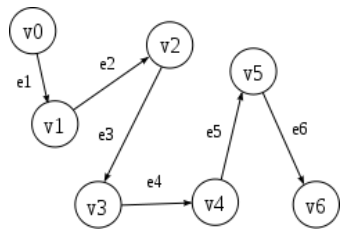
\includegraphics[width=8cm, height=4cm]{graf1} 
		\label{fig:graf1} 
	\end{figure}
	
Graf memiliki banyak jenis, jenis-jenis graf ini didasarkan pada ada tidaknya \textit{loop} pada suatu graf dan sisi pada graf yang mempunyai orientasi arah. Berdasarkan ada tidaknya \textit{loop} pada suatu graf digolongkan menjadi dua jenis :
\begin{enumerate}
	\item Graf Sederhana
	
	Graf ini tidak mempunyai sisi ganda.
	\item Graf tak-sederhana
	
	Graf ini mempunyai sisi ganda.
\end{enumerate}

Berdasarkan orientasi arah pada sisi, secara umum graf dibedakan menjadi 2 jenis :
\begin{enumerate}
	\item Graf tak-berarah
	
	Graf yang sisinya tidak mempunyai arah. Pada graf ini urutan sisi tidak diperhatikan.
	\item Graf berarah
	
	Graf yang sisinya mempunyai arah. Pada graf ini urutan sisi diperhatikan. 
\end{enumerate}

Sebuah graf dinyatakan sebagai struktur data yang terdiri dari simpul dan sisi yang membangun hubungan antar simpul. Terdapat dua macam representasi graf yaitu \textit{adjacency list} dan \textit{adjacency matrix}. 
\subsection{Adjacency List}
Adjacency list merupakan bentuk representasi dari seluruh sisi dalam sebuah graf sebagai suatu senarai (\textit{linked list}). Simpul-simpul yang dihubungkan merupakan simpul-simpul yang saling terkait. Dalam implementasinya, adjacency list menggunakan \textit{hash table} untuk menghubungkan satu simpul dengan simpul lain yang saling terkait. Contoh implementasi adjacency list yaitu sebagai berikut :

 	\begin{figure} [H]
		\centering  
		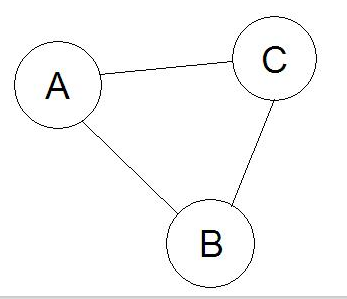
\includegraphics[width=4cm, height=4cm]{adjacencylist} 
		\caption[\textit{Undirected Cyclic Graph}]{\textit{Undirected Cyclic Graph}}
		\label{fig:GambarAL} 
	\end{figure}
	
	Graf pada gambar \ref{fig:GambarAL} dapat direpresentasikan melalui tabel \ref{tabelAL} :
	
	
	\begin{table}[H]
\centering
\caption{Tabel Representasi Adjacency List}
\begin{tabular}{|c|p{2cm}|c|}
\hline
Vertex & Adjacency & Array of Adjacent\\
\hline
a & adjacent to & b,c \\
\hline
b & adjacent to & a,c \\
\hline
c & adjacent to & a,b\\
\hline
\end{tabular}
\label{tabelAL}
\end{table}

\subsection{Adjacency Matrix}
Adjacency Matrix merupakan representasi matrix $N \times N$ yang menyatakan hubungan antar simpul dalam suatu graf. Kolom dan baris menyatakan simpul-simpul, sedangkan nilai entri dari matrix menyatakan hubungan antar simpul. Contoh implementasi adjacency matrix yaitu sebagai berikut :

\begin{figure} [H]
		\centering  
		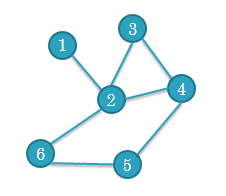
\includegraphics[width=5cm, height=4cm]{adjacencymatrix} 
		\caption[\textit{Undirected Cyclic Graph}]{\textit{Undirected Cyclic Graph}}
		\label{fig:GambarAM} 
	\end{figure}


Graf pada gambar \ref{fig:GambarAM} dapat direpresentasikan melalui tabel \ref{tabelAM} :


\begin{table}[H]
\centering
\caption{Tabel Representasi Adjacency Matrix}
\begin{tabular}{|c|c|c|c|c|c|c|}
\hline
v & 1 & 2 & 3 & 4 & 5 & 6 \\
\hline
1 & 0 & 1 & 0 & 0 & 0 & 0 \\
\hline
2 & 1 & 0 & 1 & 1 & 0 & 1 \\
\hline
3 & 0 & 1 & 0 & 1 & 0 & 0 \\
\hline
4 & 0 & 1 & 1 & 0 & 1 & 0 \\
\hline
5 & 0 & 0 & 0 & 1 & 0 & 1 \\
\hline
6 & 0 & 1 & 0 & 0 & 1 & 0 \\
\hline
\end{tabular}
\label{tabelAM}
\end{table}
	\item Melakukan analisis kebutuhan perangkat lunak
	
	
				{\bf Status :} Ada sejak rencana kerja skripsi .\\
		    {\bf Hasil :}
	\item Merancang perangkat lunak
	
	{\bf Status :} Ada sejak rencana kerja skripsi.\\
		    {\bf Hasil :}
	\item Mengimplementasikan perangkat lunak
	
	{\bf Status :} Ada sejak rencana kerja skripsi.\\
		    {\bf Hasil :}
	\item Menguji dan mensimulasikan perangkat lunak dengan parameter yang digunakan untuk mensimulasikan pertumbuhan wirausaha.
	
	{\bf Status :} Ada sejak rencana kerja skripsi.\\
		    {\bf Hasil :}
	\item Mengambil kesimpulan tentang model yang telah dikembangkan
	
	{\bf Status :} Ada sejak rencana kerja skripsi.\\
		    {\bf Hasil :}
	\item Menulis dokumen skripsi
	
	{\bf Status :} Ada sejak rencana kerja skripsi.\\
		    {\bf Hasil :}
\end{enumerate}

\footnotetext{Nawangpalupi, C.B., et.al. GEM 2013. Indonesian Report. 2013.}

\section{Pencapaian Rencana Kerja}
Langkah-langkah kerja yang berhasil diselesaikan dalam Skripsi 1 ini adalah sebagai berikut:
\begin{enumerate}
\item Melakukan studi literatur tentang GEM (Global Entrepreneurship Monitor).
\item Mempelajari teori tentang \textit{Cellular Automata} yang khususnya \textit{Entrepreneur Cellular Automata}.
\item Mempelajari teori tentang graf.
\item
\end{enumerate}



\section{Kendala yang Dihadapi}
%TULISKAN BAGIAN INI JIKA DOKUMEN ANDA TIPE A ATAU C
Kendala - kendala yang dihadapi selama mengerjakan skripsi :
\begin{itemize}
	%\item Terlalu banyak melakukan prokratinasi
	\item Terlalu banyak godaan berupa hiburan (gadget, film, dll)
	\item Skripsi diambil bersamaan dengan banyak mata kuliah yang masing-masing memiliki tugas besar.
	\item Mengalami kesulitan pada saat mempelajari struktur ECA dan perhitungannya.
\end{itemize}

\vspace{1cm}
\centering Bandung, \tanggal\\
\vspace{2cm} \nama \\ 
\vspace{1cm}

Menyetujui, \\
\ifdefstring{\jumpemb}{2}{
\vspace{1.5cm}
\begin{centering} Menyetujui,\\ \end{centering} \vspace{0.75cm}
\begin{minipage}[b]{0.45\linewidth}
% \centering Bandung, \makebox[0.5cm]{\hrulefill}/\makebox[0.5cm]{\hrulefill}/2013 \\
\vspace{2cm} Nama: \pembA \\ Pembimbing Utama
\end{minipage} \hspace{0.5cm}
\begin{minipage}[b]{0.45\linewidth}
% \centering Bandung, \makebox[0.5cm]{\hrulefill}/\makebox[0.5cm]{\hrulefill}/2013\\
\vspace{2cm} Nama: \pemB \\ Pembimbing Pendamping
\end{minipage}
\vspace{0.5cm}
}{
% \centering Bandung, \makebox[0.5cm]{\hrulefill}/\makebox[0.5cm]{\hrulefill}/2013\\
\vspace{2cm} Nama: \pembA \\ Pembimbing Tunggal
}
\end{document}

